\documentclass[11pt]{article}
\usepackage[T1]{fontenc}
\usepackage[utf8]{inputenc}
\usepackage[margin=1in]{geometry}
\usepackage{amsmath,amssymb,amsthm,mathtools,booktabs,array}
\usepackage{microtype}
\usepackage{tikz}
\usetikzlibrary{positioning}
\usepackage[numbers,sort&compress]{natbib}
\usepackage[colorlinks=true,allcolors=blue]{hyperref}
\newcommand{\R}{\mathbb{R}}
\newcommand{\Q}{\mathbb{Q}}
\newcommand{\ER}{\exists\mathbb{R}}
\newcommand{\NP}{\mathsf{NP}}
\newcommand{\PSPACE}{\mathsf{PSPACE}}
\newcommand{\RPF}{\textnormal{\textsc{RPF}}}
\newcommand{\ACPF}{\textnormal{\textsc{ACPF}}}
\newcommand{\ETRINV}{\textnormal{\textsc{ETR-INV}}}
\newcommand{\power}{\mathcal{P}}
\newcommand{\comp}[1]{\overline{#1}}
\newtheorem{theorem}{Theorem}[section]
\newtheorem{lemma}[theorem]{Lemma}
\newtheorem{proposition}[theorem]{Proposition}
\newtheorem{corollary}[theorem]{Corollary}
\theoremstyle{definition}
\newtheorem{definition}[theorem]{Definition}
\theoremstyle{remark}
\newtheorem{remark}[theorem]{Remark}

\title{Exact Feasibility of Resistive and AC Power Networks}
\author{}
\date{}
\begin{document}
\maketitle
\begin{abstract}
We prove that feasibility of a resistive power network with positive voltage
intervals and signed power-injection intervals is complete for the existential
theory of the reals. The result holds on simple graphs of maximum degree three,
with conductances in $\{1,2\}$ and all interval endpoints from fixed finite sets.
The reduction implements bounded addition and inversion using voltage-pinned
buses and complement paths. It preserves the solution set by a rational
bijection whose inverse reads designated bus voltages. We transfer this
completeness result to AC networks with resistive lines and zero reactive
injections. For rational cosine limits representing real line-angle bounds
strictly below $\pi$, a polynomial encoding of cycle winding enforces the
existence of consistent real bus angles. A separate transfer covers linear
bus-angle boxes. Principal-angle limits alone allow winding solutions, but
strictly positive windows with polynomial-bit, size-dependent cosines also
give completeness. A reactive-balance identity permits one-sided
positive-width reactive intervals in all these transfers. Consequently,
polynomial-size certificates for exact
feasibility verifiable in deterministic polynomial time would imply
$\NP=\ER$.
\end{abstract}
\section{Exact feasibility and the resistive model}
\label{sec:foundations}

In a resistive network, current depends linearly on bus voltages, but power is
the product of voltage and current. This distinction makes exact feasibility a
quadratic problem even when the network has no discrete controls. We study its
complexity with interval restrictions on both voltage and net power injection.
The model concerns direct-current electrical networks; it is distinct from
the linear ``DC approximation'' of an alternating-current network.

\subsection{Input model and complexity convention}

Let $G=(N,E)$ be a finite simple undirected graph. Each line $\{i,j\}\in E$
has conductance $g_{ij}=g_{ji}\in\Q_{>0}$. Bus $i$ has voltage bounds
$0<\ell_i\le u_i$ and injection bounds $p_i^-\le p_i^+$, all rational and
finite. Its net injection at voltage vector $v\in\R^N$ is
\begin{equation}
 \power_i(v)=v_i\sum_{j:\{i,j\}\in E}g_{ij}(v_i-v_j).
 \label{eq:rpf}
\end{equation}
An injection is positive for net supply to the network and negative for net
withdrawal. An isolated bus has injection zero. The decision problem $\RPF$
asks whether
\begin{equation}
 \ell_i\le v_i\le u_i,\qquad
 p_i^-\le\power_i(v)\le p_i^+\qquad(i\in N)
 \label{eq:rpf-bounds}
\end{equation}
has a solution. Singleton intervals are allowed. We impose neither additional
line-flow limits nor a requirement that an injection be fixed whenever a
voltage is variable. Thus the input permits voltage-pinned buses with fixed
injections, variable-voltage buses with fixed injections, and buses with both
quantities in intervals. These choices are material to the reduction.

The graph and its rational data are encoded in binary. The existential
theory of the reals, denoted ETR, asks whether an existentially quantified
Boolean combination of polynomial equalities and inequalities with integer
coefficients is true. The class $\ER$ consists of decision problems reducible
to ETR by polynomial-time many-one reductions. Rational coefficients are
equivalent: each atomic constraint can have its denominators cleared using
a positive integer of polynomial bit length. We use the Turing model of
computation and the standard inclusions
\begin{equation}
 \NP\subseteq\ER\subseteq\PSPACE.
 \label{eq:complexity-inclusions}
\end{equation}
See \citet[Section 1.1]{AbrahamsenMiltzow2019} for these conventions and their
background. Exact feasibility quantifies over real solutions, not over decimal
approximations. An irrational solution alone does not rule out membership in
$\NP$: a certificate need not list rational bus voltages.

\begin{proposition}
\label{prop:rpf-membership}
The problem $\RPF$ belongs to $\ER$.
\end{proposition}
\begin{proof}
Equations~\eqref{eq:rpf}--\eqref{eq:rpf-bounds} form a conjunction of rational
polynomial inequalities of degree at most two in $|N|$ real variables.
Writing each incident-line term explicitly uses $O(|N|+|E|)$ terms and
polynomially many bits. Clearing denominators gives an ETR instance.
\end{proof}

The model respects the usual dissipation identity:
\begin{equation}
 \sum_{i\in N}\power_i(v)
 =\sum_{\{i,j\}\in E}g_{ij}(v_i-v_j)^2\ge0.
 \label{eq:dissipation}
\end{equation}
Indeed, the two terms of a line sum to $g_{ij}(v_i-v_j)^2$.
The injection intervals, rather than a separate balance equation with zero
total injection, account for these losses. In particular, permitting signed
injections does not remove physical power balance.

\subsection{The bounded arithmetic source problem}

An instance of $\ETRINV$ consists of named variables $x_1,\ldots,x_n$,
each restricted to $[1/2,2]$, and a conjunction of equations of the forms
\begin{equation}
 x=1,\qquad x+y=z,\qquad xy=1.
 \label{eq:etr-inv}
\end{equation}
Variable names in an equation may coincide. The interval restrictions are
part of feasibility, not a promise that all real solutions already lie there.
Abrahamsen, Adamaszek, and Miltzow prove this problem $\ER$-complete
\citep[Definition 5 and Theorem 7 of the STOC/arXiv version]{AbrahamsenEtAl2018}.
The journal version is \citet{AbrahamsenEtAl2022}.
Replacing each equation $x=1$ by $x x=1$ preserves the solution set, since
$x>0$. Hence we use only addition and inversion equations below.
Let $S_\Phi\subseteq[1/2,2]^n$ denote the solution set of the normalized
instance $\Phi$, and let $m$ be its number of equations.
We retain all named variables, including those occurring in no equation.

\section{A bounded-degree reduction with fixed numerical data}
\label{sec:resistive}

\begin{theorem}
\label{thm:rpf-complete}
The problem $\RPF$ is $\ER$-complete. Hardness holds for simple graphs with
maximum degree three, conductances in $\{1,2\}$, voltage intervals in
\[
 \bigl\{[1/2,2],\ [1,1],\ [1,4]\bigr\},
\]
and injection intervals in
\[
 \bigl\{[-85,85],\ [-1/2,-1/2],\ [1/2,1/2],\
 [-5/2,-5/2],\ [-1,-1]\bigr\}.
\]
For an instance of $\ETRINV$ with $n$ named variables and $m$ equations,
the reduction constructs at most $n+16m$ buses and $18m$ lines.
\end{theorem}

The construction uses a voltage-pinned bus to impose a linear relation on
its neighbors, and one variable-voltage bus to impose inversion.
Copying values along paths keeps the degree bounded even when a variable
occurs arbitrarily often. Throughout this section, a \emph{free injection}
means the fixed interval $[-85,85]$, not an unbounded or omitted constraint.

\subsection{Pinned buses and the supply of distinct value copies}
\label{subsec:copies}

A \emph{value bus} has voltage interval $[1/2,2]$ and free injection.
A \emph{pinned bus} has voltage $1$ and a specified injection $p$.
If its distinct neighbors carry voltages $a_1,\ldots,a_d$ with conductances
$h_1,\ldots,h_d$, its equation is
\begin{equation}
 \sum_{r=1}^d h_r(1-a_r)=p.
 \label{eq:pinned}
\end{equation}
In particular, a pinned bus $C$ with injection $-1/2$ and two unit-conductance
lines enforces $a+b=5/2$. Write $\comp{x}=5/2-x$; the map $x\mapsto\comp{x}$
is an involution of $[1/2,2]$.

For each variable $x$ begin with a value bus $X_x$. Successively extending a
path
\begin{equation}
 X_x\mathbin{\text{---}} C_1\mathbin{\text{---}}\comp{X}_x\mathbin{\text{---}}C_2\mathbin{\text{---}}X'_x\mathbin{\text{---}}\cdots
 \label{eq:copy-chain}
\end{equation}
supplies alternating voltages $x,\comp{x},x,\ldots$.
Each $C_r$ has voltage $1$, injection $-1/2$, and exactly its two path lines.
Every value bus may receive at most one further line from an equation gadget.
Here is a deterministic allocation rule. Maintain the current end of each
path, its parity (plain or complemented), and whether its one gadget slot is
unused. On a request for a copy, extend the path until the end has the requested
parity and an unused slot; allocate that slot and continue from this end for
the next request. Each extension adds one pinned bus, one value bus, and two
lines. At most two extensions are needed per request. All requested copies
are distinct, even if they represent the same variable in the same equation.
Unused named variables retain their single isolated bus $X_x$.

\subsection{Addition and inversion gadgets}

For $x+y=z$, introduce a pinned bus $A$ with injection $1/2$ and three
unit-conductance lines to fresh requested copies of $x$, $y$, and
$\comp{z}$. Its equation is
\[
 (1-x)+(1-y)+(1-\comp{z})=1/2
 \quad\Longleftrightarrow\quad x+y=z.
\]
For $x+x=z$ the two plain copies of $x$ are distinct buses. The same allocation
rule covers $x+y=x$ and $x+x=x$; such equations are correctly infeasible in
the positive source interval.

For $xy=1$, introduce buses $I,W,C_I,D$ with the data in
Table~\ref{tab:inversion}. Request three distinct complemented value buses:
two for $x$ and one for $y$. Connect them as in Figure~\ref{fig:inversion}.
If $x=y$, all three still have distinct bus identities.

\begin{table}[htbp]
\centering
\begin{tabular}{@{}clll@{}}
\toprule
Bus & Voltage interval & Injection interval & Neighbors (conductance)\\
\midrule
$I$ & $[1/2,2]$ & $[-1,-1]$ & $W$ (1), $C_I$ (1)\\
$W$ & $[1,4]$ & $[-85,85]$ & $I$ (1), $D$ (1)\\
$C_I$ & $[1,1]$ & $[-1/2,-1/2]$ & $I$ (1), first $\comp{x}$ copy (1)\\
$D$ & $[1,1]$ & $[-5/2,-5/2]$ & $W$ (1), second $\comp{x}$ copy (2), $\comp{y}$ copy (1)\\
\bottomrule
\end{tabular}
\caption{The four new buses for an inversion equation $xy=1$.}
\label{tab:inversion}
\end{table}

\begin{figure}[htbp]
\centering
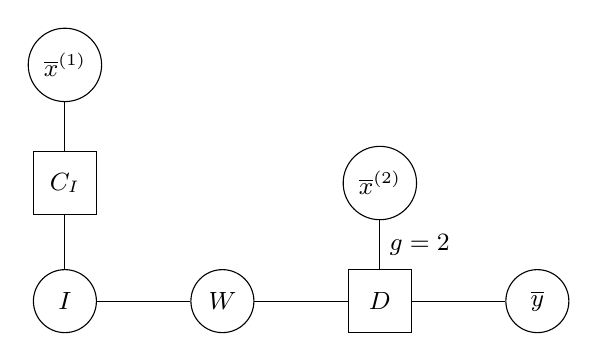
\begin{tikzpicture}[every node/.style={font=\small},
 bus/.style={circle,draw,minimum size=8mm},
 pin/.style={rectangle,draw,minimum size=8mm}]
\node[bus] (I) at (0,0) {$I$};
\node[bus] (W) at (2,0) {$W$};
\node[pin] (D) at (4,0) {$D$};
\node[pin] (C) at (0,1.5) {$C_I$};
\node[bus] (x1) at (0,3) {$\comp{x}^{(1)}$};
\node[bus] (x2) at (4,1.5) {$\comp{x}^{(2)}$};
\node[bus] (y) at (6,0) {$\comp{y}$};
\draw (x1)--(C)--(I)--(W)--(D)--(y);
\draw (D)--node[right] {$g=2$}(x2);
\end{tikzpicture}
\caption{Inversion gadget. Squares have voltage $1$; the three upper or
rightmost value copies belong to variable paths, whose lines are omitted.
Every unmarked line has conductance $1$. Superscripts distinguish buses,
not numerical values.}
\label{fig:inversion}
\end{figure}

The equation at $C_I$ gives
\[
 (1-v_I)+(1-\comp{x})=-1/2,
 \qquad\text{hence }v_I=x.
\]
The injection equation at $I$ is therefore
\begin{equation}
 x\bigl[(x-v_W)+(x-1)\bigr]=-1,
 \qquad v_W=2x-1+1/x.
 \label{eq:inversion-I}
\end{equation}
Division is valid because $x\ge1/2$. At $D$ the equation reads
\begin{equation}
 (1-v_W)+2(1-\comp{x})+(1-\comp{y})=-5/2
 \quad\Longleftrightarrow\quad y=v_W-2x+1.
 \label{eq:inversion-D}
\end{equation}
Together these equations imply $y=1/x$.

Conversely, if $x,y\in[1/2,2]$ and $xy=1$, set $v_I=x$ and
$v_W=h(x):=2x-1+1/x$. Both pinned-bus equations and the injection equation
at $I$ then hold. The voltage bound on $W$ is valid: on $[1/2,2]$,
$h'(x)=2-x^{-2}$ and $h''(x)=2x^{-3}>0$, so its minimum is
$2\sqrt{2}-1$ at $1/\sqrt{2}$ and its maximum is the larger endpoint value,
$h(2)=7/2$. Thus
\begin{equation}
 1<2\sqrt{2}-1\le v_W\le7/2<4.
 \label{eq:W-range}
\end{equation}

\subsection{The complete network and proof of equivalence}

Construct all variable paths and equation gadgets with the allocation rule
above. Path value buses have at most two path lines and one gadget line.
Path pinned buses and $C_I$ have degree two; addition buses and $D$ have
degree three; $I$ and $W$ have degree two. Distinct requested copies and fresh
gadget buses prevent loops and parallel edges. Consequently $G$ is simple and
its maximum degree is three.

Every bus voltage belongs to $[1/2,4]$ and every conductance is at most $2$.
For every voltage vector in the prescribed box, not just the intended
solutions, a free-injection bus satisfies
\begin{equation}
 |\power_i(v)|
 \le v_i\sum_{j:\{i,j\}\in E}g_{ij}|v_i-v_j|
 \le 4\cdot3\cdot2\cdot\frac72=84<85.
 \label{eq:free-bound}
\end{equation}
The free-injection intervals therefore add no restriction inside that box.

\begin{lemma}
\label{lem:reduction-equivalence}
The constructed network is feasible if and only if $S_\Phi\ne\varnothing$.
More precisely, restriction to $(v_{X_x})_{x= x_1,\ldots,x_n}$ is a bijection
from its feasible voltage set onto $S_\Phi$.
\end{lemma}
\begin{proof}
Given a feasible voltage vector, put $x=v_{X_x}$ for each named variable.
Every path pinned bus has exactly its two prescribed neighbors, so its
equation forces successive values to be complementary. Every requested copy
thus has its specified value. The addition equation yields $x+y=z$; equations
\eqref{eq:inversion-I}--\eqref{eq:inversion-D} yield $xy=1$. This recovers a
point of $S_\Phi$.

Conversely, given a point of $S_\Phi$, assign alternating values $x$ and
$5/2-x$ along each variable path, voltage $1$ to every pinned bus, and
$v_I=x$, $v_W=2x-1+1/x$ in each inversion gadget. The preceding algebra
verifies every fixed-injection equation. The voltage bounds follow from the
source interval and~\eqref{eq:W-range}; the remaining injection bounds follow
from~\eqref{eq:free-bound}. An isolated $X_x$ has injection zero and retains
exactly the unconstrained source coordinate $x\in[1/2,2]$.

Finally all bus voltages have been uniquely determined by the recovered
source coordinates: path values alternate, pinned values are fixed, and
\eqref{eq:inversion-I} determines $W$. These two maps are inverse bijections.
\end{proof}

\begin{proof}[Proof of Theorem~\ref{thm:rpf-complete}]
Each equation requests exactly three value copies. With at most two path
extensions per request, the paths contribute at most $12m$ new buses and
$12m$ lines in addition to the $n$ initial buses. An addition adds one
further bus and three lines; an inversion adds four further buses and six
lines. Hence the stated bounds $n+16m$ and $18m$ hold, including unused
variables. All numerical data are exactly those displayed in the theorem.
The number of objects is linear in $n+m$; encoding their indices uses
$O((n+m)\log(n+m+2))$ bits, and the construction is polynomial-time.
Lemma~\ref{lem:reduction-equivalence} and $\ER$-completeness of $\ETRINV$
give hardness. Proposition~\ref{prop:rpf-membership} gives membership.
\end{proof}

\begin{proposition}[Preservation of the solution set]
\label{prop:rational-bijection}
The extension map from source solutions to feasible network voltages in
Lemma~\ref{lem:reduction-equivalence} is a homeomorphism whose forward and
inverse coordinate functions are rational with rational coefficients.
Its inverse is restriction to the buses $X_x$, a coordinate projection.
\end{proposition}
\begin{proof}
The extension map has coordinate functions $x$, $5/2-x$, $1$, and
$2x-1+1/x$. They are rational and continuous because $x\ge1/2$.
The inverse projection is linear and continuous. The statement also holds
for empty solution sets and for unused source coordinates.
\end{proof}

\begin{corollary}
\label{cor:rpf-np}
If $\RPF$ belongs to $\NP$, then $\NP=\ER$. In particular, unless these
classes coincide, not every feasible rational instance has a polynomial-size
certificate verifiable in deterministic polynomial time. The problem belongs
to $\PSPACE$.
\end{corollary}
\begin{proof}
By completeness every problem in $\ER$ reduces to $\RPF$. Membership of
$\RPF$ in $\NP$ would imply $\ER\subseteq\NP$, and
\eqref{eq:complexity-inclusions} gives equality. The certificate formulation
is the definition of $\NP$; the space upper bound follows from the same
inclusions.
\end{proof}

The fixed-data conclusion is stronger than a claim that large numerical
coefficients can be encoded economically: all numerical choices in the
hard instances come from finite sets independent of instance size. Their
combinatorial incidence pattern carries the growing input. The theorem uses
general graphs and signed injection intervals; it makes no assertion here
about a load-only model or a tree restriction.

\section{AC feasibility and the meaning of angle limits}
\label{sec:ac}

The resistive result transfers to an AC model with zero reactive injections.
The transfer requires a consistent real angle at every bus: small principal
angle differences on individual lines need not fit together around a cycle.
We first encode this consistency without transcendental constraints. The
encoding works for every line limit strictly below $\pi$, including limits
larger than $\pi/2$.

\subsection{The AC input model}

Write $\mathrm{i}^2=-1$. On a simple undirected graph, line $\{i,j\}$ has
series admittance $y_{ij}=g_{ij}+\mathrm{i}b_{ij}$, where
$g_{ij}\in\Q_{\ge0}$, $b_{ij}\in\Q$, and $y_{ij}\ne0$. Bus $i$ may have a
shunt admittance $s_i=h_i+\mathrm{i}t_i$, with $h_i\in\Q_{\ge0}$ and
$t_i\in\Q$; absence of a shunt means $h_i=t_i=0$. These are reciprocal
series lines without transformers or phase shifters. A line-charging shunt
at a line endpoint may be included in that bus's shunt sum.
Let $U_i=v_i\exp(\mathrm{i}\theta_i)$, with $v_i>0$ and
$\theta_i\in\R$. With injection positive into the network, the equations are
\begin{equation}
 I_i=s_iU_i+\sum_{j:\{i,j\}\in E}y_{ij}(U_i-U_j),\qquad
 P_i+\mathrm{i}Q_i=U_i\overline{I_i}.
 \label{eq:complex-power}
\end{equation}
The input gives positive rational magnitude bounds $\ell_i\le v_i\le u_i$
and finite rational intervals $[p_i^-,p_i^+]$, $[q_i^-,q_i^+]$ for $P_i,Q_i$.
Singleton intervals are allowed independently for these three quantities.
Every line also has a rational number $c_{ij}\in(-1,1]$, representing
$\gamma_{ij}=\arccos c_{ij}\in[0,\pi)$, and the constraint
\begin{equation}
 |\theta_i-\theta_j|\le\gamma_{ij}.
 \label{eq:real-angle-limit}
\end{equation}
The problem $\ACPF$ asks for $v\in\R_{>0}^N$ and $\theta\in\R^N$ satisfying
these equations and bounds. The rational input contains $c_{ij}$, not an
approximation to $\gamma_{ij}$. Angles may be shifted by a common constant
on each connected component; an optional reference angle zero per component
only fixes this freedom.

For later use, write $U_i=e_i+\mathrm{i}f_i$ and introduce a positive magnitude
variable $r_i$. Define
\begin{equation}
 H_{ij}=e_ie_j+f_if_j,\qquad D_{ij}=f_ie_j-e_if_j.
 \label{eq:dot-cross}
\end{equation}
Thus $D_{ij}=\operatorname{Im}(U_i\overline{U_j})=-D_{ji}$.
Expanding~\eqref{eq:complex-power} gives the polynomial expressions
\begin{align}
 P_i&=h_ir_i^2+\sum_j\bigl[g_{ij}(r_i^2-H_{ij})-b_{ij}D_{ij}\bigr],
 \label{eq:rect-P}\\
 Q_i&=-t_ir_i^2+\sum_j\bigl[-b_{ij}(r_i^2-H_{ij})-g_{ij}D_{ij}\bigr],
 \label{eq:rect-Q}\\
 r_i^2&=e_i^2+f_i^2,\qquad \ell_i\le r_i\le u_i.
 \label{eq:rect-magnitude}
\end{align}
Here and below, line sums run over neighbors of $i$. All these constraints
have rational coefficients and degree at most two.

\subsection{A polynomial encoding of real angle lifts}

For two nonzero phasors with non-antipodal directions, let
$\delta_{ij}\in(-\pi,\pi)$ be the principal argument of
$U_i\overline{U_j}$. The principal-angle limit
$|\delta_{ij}|\le\gamma_{ij}$ is exactly
\begin{equation}
 H_{ij}\ge c_{ij}r_ir_j.
 \label{eq:cosine-test}
\end{equation}
Indeed, $H_{ij}/(r_ir_j)=\cos\delta_{ij}$, and cosine decreases on $[0,\pi]$.
Since $c_{ij}>-1$, antipodal directions are excluded. The positive variables
$r_i$ make squaring unnecessary, so the same test covers negative cosines.
Condition~\eqref{eq:cosine-test} alone does not encode~\eqref{eq:real-angle-limit}.

\begin{lemma}[Short-arc crossing count]
\label{lem:crossing}
Let $U_i,U_j\ne0$ have non-antipodal directions, and traverse the short
oriented arc from $U_j/|U_j|$ to $U_i/|U_i|$. Its signed crossing count of
the positive real ray, counting arrival from the open lower half-plane as
$+1$ and departure into that half-plane as $-1$, is
\begin{equation}
 k_{ij}=\begin{cases}
 1,& f_j<0\le f_i\ \text{and }D_{ij}>0,\\
 -1,& f_i<0\le f_j\ \text{and }D_{ij}<0,\\
 0,&\text{otherwise}.
 \end{cases}
 \label{eq:crossing-rule}
\end{equation}
In particular $k_{ji}=-k_{ij}$. If $\alpha_i,\alpha_j\in[0,2\pi)$ are the
arguments of the endpoints, then
\begin{equation}
 \delta_{ij}=\alpha_i-\alpha_j+2\pi k_{ij}.
 \label{eq:crossing-identity}
\end{equation}
\end{lemma}
\begin{proof}
Put $a=\alpha_i-\alpha_j\in(-2\pi,2\pi)$.
If $a< -\pi$, then $\delta_{ij}=a+2\pi\in(0,\pi)$.
Necessarily $\alpha_j>\pi$ and $\alpha_i<\pi$, so
$f_j<0\le f_i$, and $D_{ij}=r_ir_j\sin\delta_{ij}>0$.
Conversely, $f_j<0\le f_i$ implies $\alpha_j\in(\pi,2\pi)$ and
$\alpha_i\in[0,\pi]$, hence $a<0$. Within $(-2\pi,0)$ the additional
condition $\sin a>0$ holds exactly when $a< -\pi$.
Thus the first case of~\eqref{eq:crossing-rule} is precisely $a< -\pi$.
Reversing $i,j$ proves that its second case is precisely $a>\pi$.
The remaining case has $|a|<\pi$, including $a=0$, and needs no wrap.
The equalities $a=\pm\pi$ are excluded by the non-antipodal hypothesis.
This proves~\eqref{eq:crossing-identity} and reversal symmetry. It also
checks the axis convention: argument zero belongs to the closed upper
half-plane; argument $\pi$ does too, but the determinant sign prevents
counting a crossing of the negative real ray.
\end{proof}

Fix one orientation $j\to i$ for every line. For any directed traversal of
a cycle $C$, write $\varepsilon_{C,ij}=1$ if it traverses that line in its
chosen orientation and $-1$ if it traverses it in reverse. Telescoping the
$\alpha$ terms in~\eqref{eq:crossing-identity} gives
\begin{equation}
 \sum_{\{i,j\}\in C}\varepsilon_{C,ij}\delta_{ij}
 =2\pi\sum_{\{i,j\}\in C}\varepsilon_{C,ij}k_{ij}.
 \label{eq:cycle-winding}
\end{equation}
The integer on the right after division by $2\pi$ is the winding number.

\begin{lemma}[Real-angle lift criterion]
\label{lem:lift}
Suppose~\eqref{eq:cosine-test} holds on every line. There are real angles
$\theta_i$ representing the phasors and satisfying~\eqref{eq:real-angle-limit}
if and only if
\begin{equation}
 \sum_{\{i,j\}\in C}\varepsilon_{C,ij}k_{ij}=0
 \label{eq:zero-winding}
\end{equation}
for each fundamental cycle of a spanning forest of $G$.
\end{lemma}
\begin{proof}
For a real lift within the limits, both $\theta_i-\theta_j$ and
$\delta_{ij}$ belong to $(-\pi,\pi)$ and represent the same argument.
They are therefore equal, and their sum around every cycle is zero.
Equation~\eqref{eq:cycle-winding} proves necessity.
Conversely choose one argument at a root of each tree of the forest and
extend $\theta$ along its edges by $\theta_i-\theta_j=\delta_{ij}$.
These angles represent the given phasors. Each non-tree edge and its
unique forest path form a fundamental cycle. Its zero sum in
\eqref{eq:cycle-winding} forces the same difference equation on that edge.
Every line difference is thus its principal difference and satisfies its limit.
\end{proof}

\begin{theorem}
\label{thm:ac-membership}
The problem $\ACPF$ belongs to $\ER$ for rational cosine limits
$c_{ij}\in(-1,1]$.
\end{theorem}
\begin{proof}
Use variables $e_i,f_i,r_i$ subject to~\eqref{eq:rect-magnitude}, the injection
intervals applied to~\eqref{eq:rect-P}--\eqref{eq:rect-Q}, and
\eqref{eq:cosine-test}. For each oriented line introduce a real $k_{ij}$ and
encode~\eqref{eq:crossing-rule} by a Boolean combination of polynomial
comparisons: either its first condition and $k_{ij}=1$, or its second
condition and $k_{ij}=-1$, or the negations of both conditions and $k_{ij}=0$.
Add~\eqref{eq:zero-winding} for the fundamental cycles.
Lemmas~\ref{lem:crossing}--\ref{lem:lift} prove equivalence to real-angle
feasibility. There are $O(|N|+|E|)$ variables and at most
$|E|-|N|+\kappa$ fundamental cycles, where $\kappa$ is the number of
components. Each cycle has at most $|N|$ edges. Consequently the Boolean
formula and its rational coefficients have polynomial encoding length.
All quantified variables are real; the three-valued crossing variables
require no additional integer quantifier.
\end{proof}

\subsection{Zero reactive injection and the hardness transfer}

For purely resistive lines with $g_{ij}>0$ and no shunts, the polar form of
\eqref{eq:rect-P}--\eqref{eq:rect-Q} is
\begin{align}
 P_i&=\sum_j g_{ij}\bigl(v_i^2-v_iv_j\cos(\theta_i-\theta_j)\bigr),
 \label{eq:resistive-ac-P}\\
 Q_i&=-\sum_j g_{ij}v_iv_j\sin(\theta_i-\theta_j).
 \label{eq:resistive-ac-Q}
\end{align}

\begin{lemma}[Equal angles under a real lift]
\label{lem:equal-angles}
In a purely resistive, shunt-free network, suppose $v_i>0$, $Q_i=0$ at
every bus, and $|\theta_i-\theta_j|<\pi$ on every line. Then angles are
constant on each connected component. The active injections are exactly
$\power_i(v)$ from~\eqref{eq:rpf}. Conversely, every positive resistive
voltage profile extends to an AC profile with these injections and $Q=0$
by taking all angles zero.
\end{lemma}
\begin{proof}
Multiply~\eqref{eq:resistive-ac-Q} by $-\theta_i$ and sum over buses.
Pairing the two contributions of each line yields
\begin{equation}
 0=-\sum_i\theta_i Q_i
 =\sum_{\{i,j\}\in E}g_{ij}v_iv_j
 (\theta_i-\theta_j)\sin(\theta_i-\theta_j).
 \label{eq:angle-energy}
\end{equation}
Each summand is nonnegative, and $t\sin t>0$ for $0<|t|<\pi$.
Since $g_{ij}v_iv_j>0$, every line difference is zero. Substitution in
\eqref{eq:resistive-ac-P} gives~\eqref{eq:rpf}. The converse follows directly
from~\eqref{eq:resistive-ac-P}--\eqref{eq:resistive-ac-Q}.
\end{proof}

The sine balance in~\eqref{eq:resistive-ac-Q} is also the equilibrium equation
of a weighted oscillator network; see \citet{DorflerEtAl2013} for this
connection and cohesive-angle analysis. The elementary identity
\eqref{eq:angle-energy} supplies the exact statement needed here, with real
bus angles and line differences strictly below $\pi$. It does not require
strictly positive cosine or a stability assumption.

\begin{theorem}
\label{thm:ac-complete}
The problem $\ACPF$ is $\ER$-complete. Hardness holds on simple graphs of
maximum degree three, with $b_{ij}=h_i=t_i=0$, $q_i^-=q_i^+=0$ at every bus,
$c_{ij}=0$ on every line, and the fixed finite conductance, magnitude, and
active-injection data of Theorem~\ref{thm:rpf-complete}.
\end{theorem}
\begin{proof}
Take the resistive instance of Theorem~\ref{thm:rpf-complete}, retain its
graph and data, and add the stated AC data. The cosine input zero represents
the real-angle limit $\pi/2$. Lemma~\ref{lem:equal-angles} proves equivalence
in both directions, and Theorem~\ref{thm:ac-membership} proves membership.
\end{proof}

Thus $\ACPF\in\NP$ would imply $\NP=\ER$. This conclusion concerns the
specified AC model with variable magnitudes and resistive lines. It does not
classify the lossless, fixed-magnitude model, whose nonlinear variables are
angles alone.

\begin{corollary}[One-sided reactive intervals]
\label{cor:one-sided-reactive}
Theorem~\ref{thm:ac-complete} remains true if every reactive-injection
interval $[0,0]$ is replaced by the positive-width interval $[0,1]$.
More generally, in a purely resistive, shunt-free network, requiring all
reactive injections to be nonnegative, or all to be nonpositive, forces
each of them to be zero.
\end{corollary}
\begin{proof}
Antisymmetry of the sine terms in~\eqref{eq:resistive-ac-Q} gives
$\sum_i Q_i=0$. Numbers of one common weak sign with zero sum all vanish.
Conversely, zero belongs to $[0,1]$, so the feasible set is unchanged.
\end{proof}

The same replacement applies to the two restricted AC formulations below.
This removes the need to specify singleton reactive intervals, while the
network identity still enforces exact zero reactive injections. It is a
one-sided saturation argument, not a robustness assertion for symmetric
intervals $[-\varepsilon,\varepsilon]$.

\subsection{Principal angles: a counterexample and a positive-window result}
\label{subsec:principal}

Define \emph{principal-angle AC feasibility} by
\eqref{eq:rect-P}--\eqref{eq:cosine-test} and the injection intervals, without
the cycle equations~\eqref{eq:zero-winding}. This is a polynomial feasibility
problem and hence belongs to $\ER$. The distinction from $\ACPF$ is material.

\begin{proposition}[Winding prevents an unrestricted transfer]
\label{prop:winding-counterexample}
On a unit-conductance $n$-cycle, $n\ge3$, the phasors
$U_k=\exp(2\pi\mathrm{i}k/n)$ have unit magnitudes and satisfy
\begin{equation}
 Q_k=0,\qquad P_k=2\bigl(1-\cos(2\pi/n)\bigr)>0.
 \label{eq:cycle-profile}
\end{equation}
Their principal line differences have absolute value $2\pi/n$ and winding
number one. Consequently, for every fixed rational $c\in(-1,1)$ there is a
rational-data instance with line cosine limit $c$ that is principal-angle
AC feasible but whose corresponding resistive instance is infeasible.
\end{proposition}
\begin{proof}
At each bus, the two sine terms in~\eqref{eq:resistive-ac-Q} cancel and the
cosine terms coincide, giving~\eqref{eq:cycle-profile}. The oriented sum
around the cycle is $2\pi$, so Lemma~\ref{lem:lift} excludes a real lift
with these principal differences. Given $c<1$, choose $n\ge3$ large enough
that $2\pi/n\le\arccos c$. Put unit magnitude bounds and zero reactive
injections at all buses, and choose rational numbers $0<a<P_k<b$ as active
injection bounds $[a,b]$. Such numbers exist by density of $\Q$; the powers
in~\eqref{eq:cycle-profile} themselves need not be rational. The phasors
give principal-angle feasibility, whereas every resistive voltage is one
and its injection is zero, outside $[a,b]$.
For an explicit instance with singleton rational injections, take $n=4$,
$c=0$, and $[p_k^-,p_k^+]=[2,2]$.
\end{proof}

This example disproves an equal-angle implication from fixed positive
principal windows; it does not assert a complexity classification for every
such fixed-window class. At the other endpoint, the bound strictly below
$\pi$ in Lemma~\ref{lem:equal-angles} is sharp: a single unit-conductance
line with unit magnitudes and real angles $0,\pi$ has $Q=0$ and active
injection $2$ at both buses.

A positive principal window can nevertheless enforce the needed real lift
when its width is allowed to depend on the graph size.

\begin{lemma}[Small cycle budgets exclude winding]
\label{lem:small-cycle-budget}
Suppose principal angle limits $\gamma_{ij}<\pi$ satisfy
$\sum_{\{i,j\}\in C}\gamma_{ij}<2\pi$ for every fundamental cycle $C$
of some spanning forest. Then every phasor profile satisfying those limits
has a real lift satisfying the same limits.
\end{lemma}
\begin{proof}
The principal difference sum on $C$ is a multiple of $2\pi$ by
\eqref{eq:cycle-winding}. Its absolute value is at most the stated sum of
limits and therefore strictly less than $2\pi$. It must vanish.
Lemma~\ref{lem:lift} applies. In particular, every forest has this property
without any additional restriction on its limits below $\pi$.
\end{proof}

\begin{corollary}[Strictly positive principal windows]
\label{cor:principal-hardness}
Principal-angle AC feasibility is $\ER$-complete even on simple graphs of
maximum degree three with purely resistive lines, no shunts, zero reactive
injections, the fixed numerical data of Theorem~\ref{thm:rpf-complete}, and
the common cosine limit
\begin{equation}
 c_n=1-\frac{1}{n^2},\qquad n=|N|\ge2.
 \label{eq:shrinking-window}
\end{equation}
The angle window is strictly positive. Its cosine has $O(\log n)$ bits;
unlike the other data, these cosines do not belong to a fixed finite set.
\end{corollary}
\begin{proof}
For $t\in[0,\pi]$, concavity of sine on $[0,\pi/2]$ gives
$\sin(t/2)\ge t/\pi$, and therefore
$1-\cos t=2\sin^2(t/2)\ge2t^2/\pi^2$.
Writing $\gamma_n=\arccos c_n$, we obtain
$0<\gamma_n\le\pi/(\sqrt{2}n)$.
Every simple cycle has at most $n$ edges, so the sum of its limits is at
most $\pi/\sqrt{2}<2\pi$. Lemma~\ref{lem:small-cycle-budget} supplies a
real lift, and Lemma~\ref{lem:equal-angles} proves equivalence to the
resistive instance. Take that instance from Theorem~\ref{thm:rpf-complete}.
If needed, add isolated buses with magnitude bounds $[1/2,2]$ and active
injection bounds $[-85,85]$ to ensure $n\ge2$. These buses are feasible
and use the original finite alphabet. Computing~\eqref{eq:shrinking-window} takes
polynomial time. Membership follows from the rectangular formulation.
\end{proof}

\subsection{A rectangular model with bus-angle boxes}
\label{subsec:angle-box}

There is also a hardness transfer using only linear angle restrictions in
rectangular coordinates. Choose a reference bus in each connected component
and require
\begin{equation}
 e_i\ge f_i,\qquad e_i\ge-f_i\quad(i\in N),\qquad
 f_{\mathrm{ref}}=0,\quad e_{\mathrm{ref}}>0.
 \label{eq:angle-box}
\end{equation}
The positive lower magnitude bounds imply $e_i>0$, so these conditions are
exactly the angle box $\theta_i\in[-\pi/4,\pi/4]$ relative to a reference
angle zero. Their real line differences lie in $[-\pi/2,\pi/2]$.

\begin{corollary}
\label{cor:box-hardness}
The rectangular AC feasibility problem with~\eqref{eq:angle-box} is
$\ER$-complete under the same graph, admittance, magnitude, and injection
restrictions as Theorem~\ref{thm:ac-complete}, without separate line-angle
constraints. In this restricted class every feasible profile has $f_i=0$
and $e_i=v_i$ at every bus, and its feasible set is exactly the resistive
voltage set in these coordinates.
\end{corollary}
\begin{proof}
The formulation is polynomial. The box supplies real angles with the
required line differences, so Lemma~\ref{lem:equal-angles} makes them
constant on each component. Its reference angle makes that constant zero.
Conversely every feasible resistive profile with $e_i=v_i$, $f_i=0$
satisfies the box and all AC constraints.
\end{proof}

The three transfers have different input conventions. Real line limits
permit the fixed choice $c_{ij}=0$ and require the winding equations for
membership. Bus-angle boxes give a direct polynomial encoding with fixed
coefficients. Positive principal-only windows give a direct polynomial
encoding with the size-dependent cosine~\eqref{eq:shrinking-window}.
None of these equivalences assumes that small numerical reactive residuals
are exactly zero.

\bibliographystyle{plainnat}
\bibliography{references}
\end{document}
